\begin{frame}{Detector Concept}

	\vspace*{-10pt}
	\begin{figure} 
		\begin{center}
			\begin{subfigure}{0.4\textwidth}  
				\centering 
				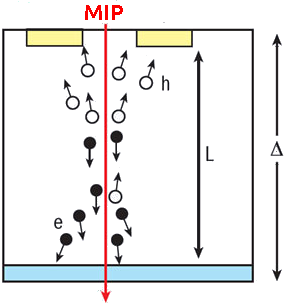
\includegraphics[height=.53\textheight]{PlanarConcept}
				\caption{planar detector}
			\end{subfigure}
			\begin{subfigure}{0.1\textwidth}  
				\centering 
				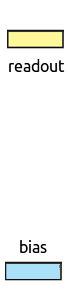
\includegraphics[height=.53\textheight]{LegendConcept}
				\vspace*{20pt}
			\end{subfigure}
			\begin{subfigure}{0.4\textwidth} 
				\centering 
				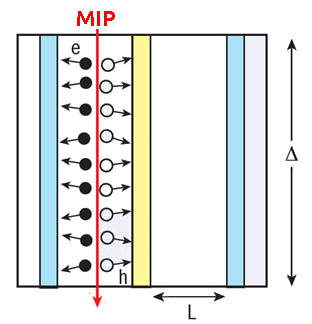
\includegraphics[height=.53\textheight]{3DConcept}
				\caption{3D detector} 	
			\end{subfigure} 
		\end{center}
	\end{figure}\vspace*{-10pt}
	
	\begin{itemize}
		\itemfill
		\item bias and readout electrode inside detector material
		\item same thickness $\Updelta$ \ra same amount of induced charge
		\item shorter drift distance L
		\item \usebeamercolor[fg]{title} \textbf{increase collected charge in detectors with limited mean free path}
	\end{itemize}
	
\end{frame}
% ================================== 2 =============================
\begin{frame}{3D Detector}
	
	\begin{figure}
		\centering
		\begin{subfigure}{0.4\textwidth}  
			\centering 
			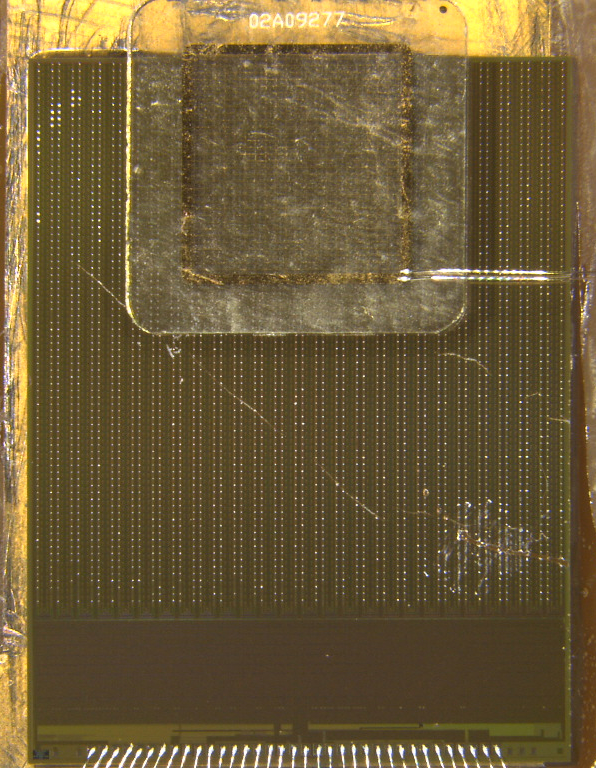
\includegraphics[height=.47\textheight]{Full3D}
			\caption{detector bonded on CMS pixel}
		\end{subfigure}
		\hspace*{10pt}
		\begin{subfigure}{0.4\textwidth} 
			\centering 
			\vspace*{.1\textheight}
			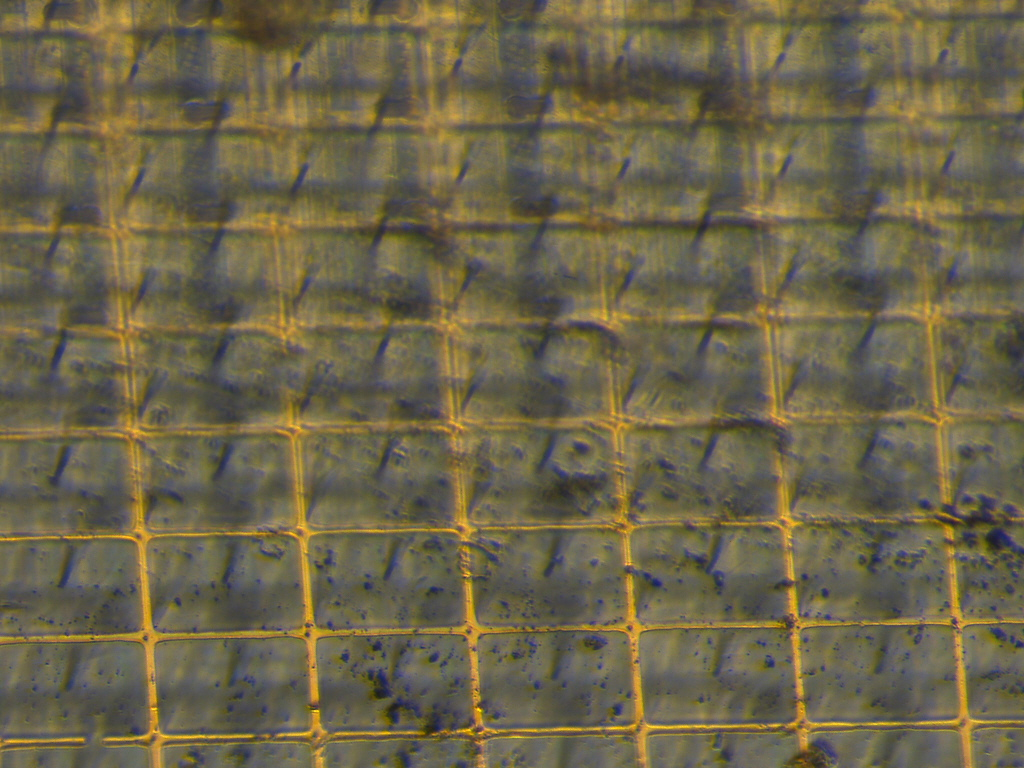
\includegraphics[height=.37\textheight]{3DCols}
			\caption{bias grid and columns}
		\end{subfigure}
	\end{figure}\vspace*{-10pt}

	\begin{itemize}
		\itemfill
		\item columns laser drilled \ra convert diamond into resistive mixture of carbon phases
		\item size of \SI{4x4}{\milli\meter}
		\item thickness of \SI{500}{\micro\meter}
		\item cell size of \SI{150x100}{\micro\meter} \ra \SI{20x30}{cells}
	\end{itemize}

\end{frame}
% ================================== 3 =============================
\begin{frame}{Raw Data}

	\vspace*{-10pt}
	\begin{figure}
		\centering
		\begin{subfigure}{0.45\textwidth}  
			\centering 
			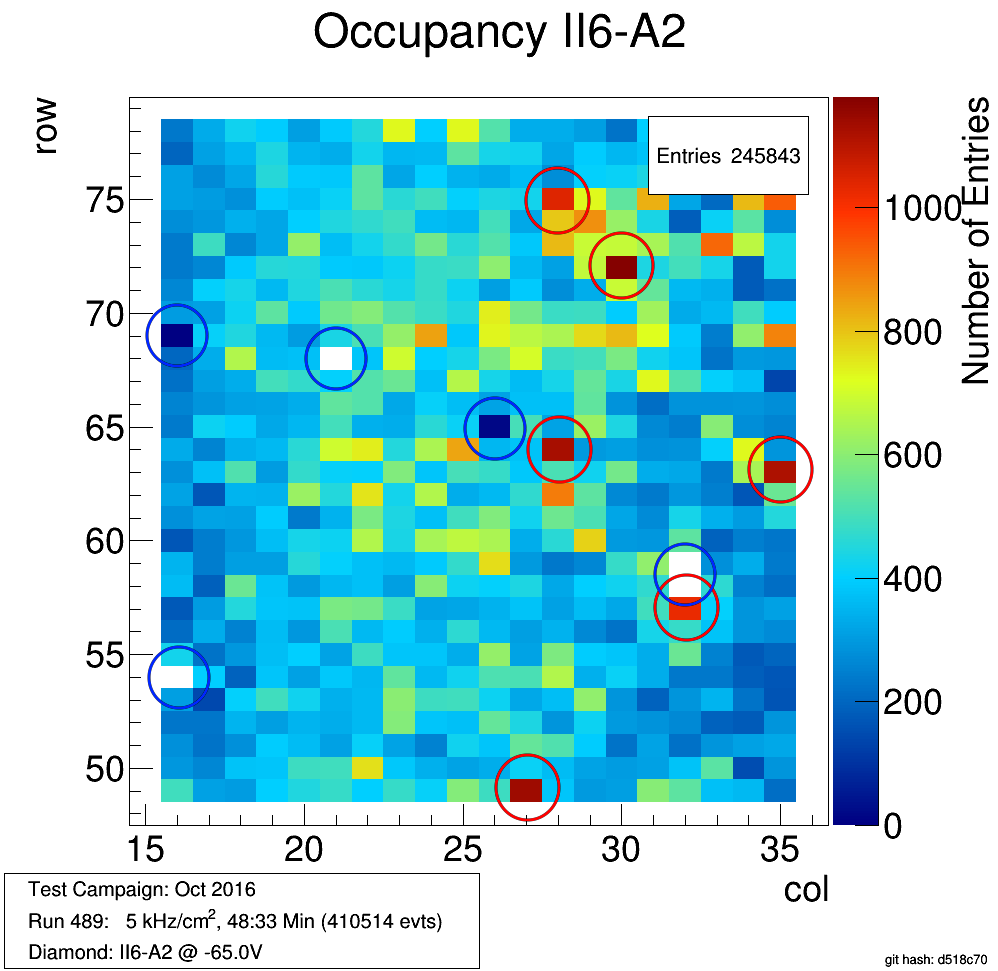
\includegraphics[height=.53\textheight]{OccRaw}
			\caption{raw hit map}
		\end{subfigure}
		\hspace*{10pt}
		\begin{subfigure}{0.45\textwidth} 
			\centering 
			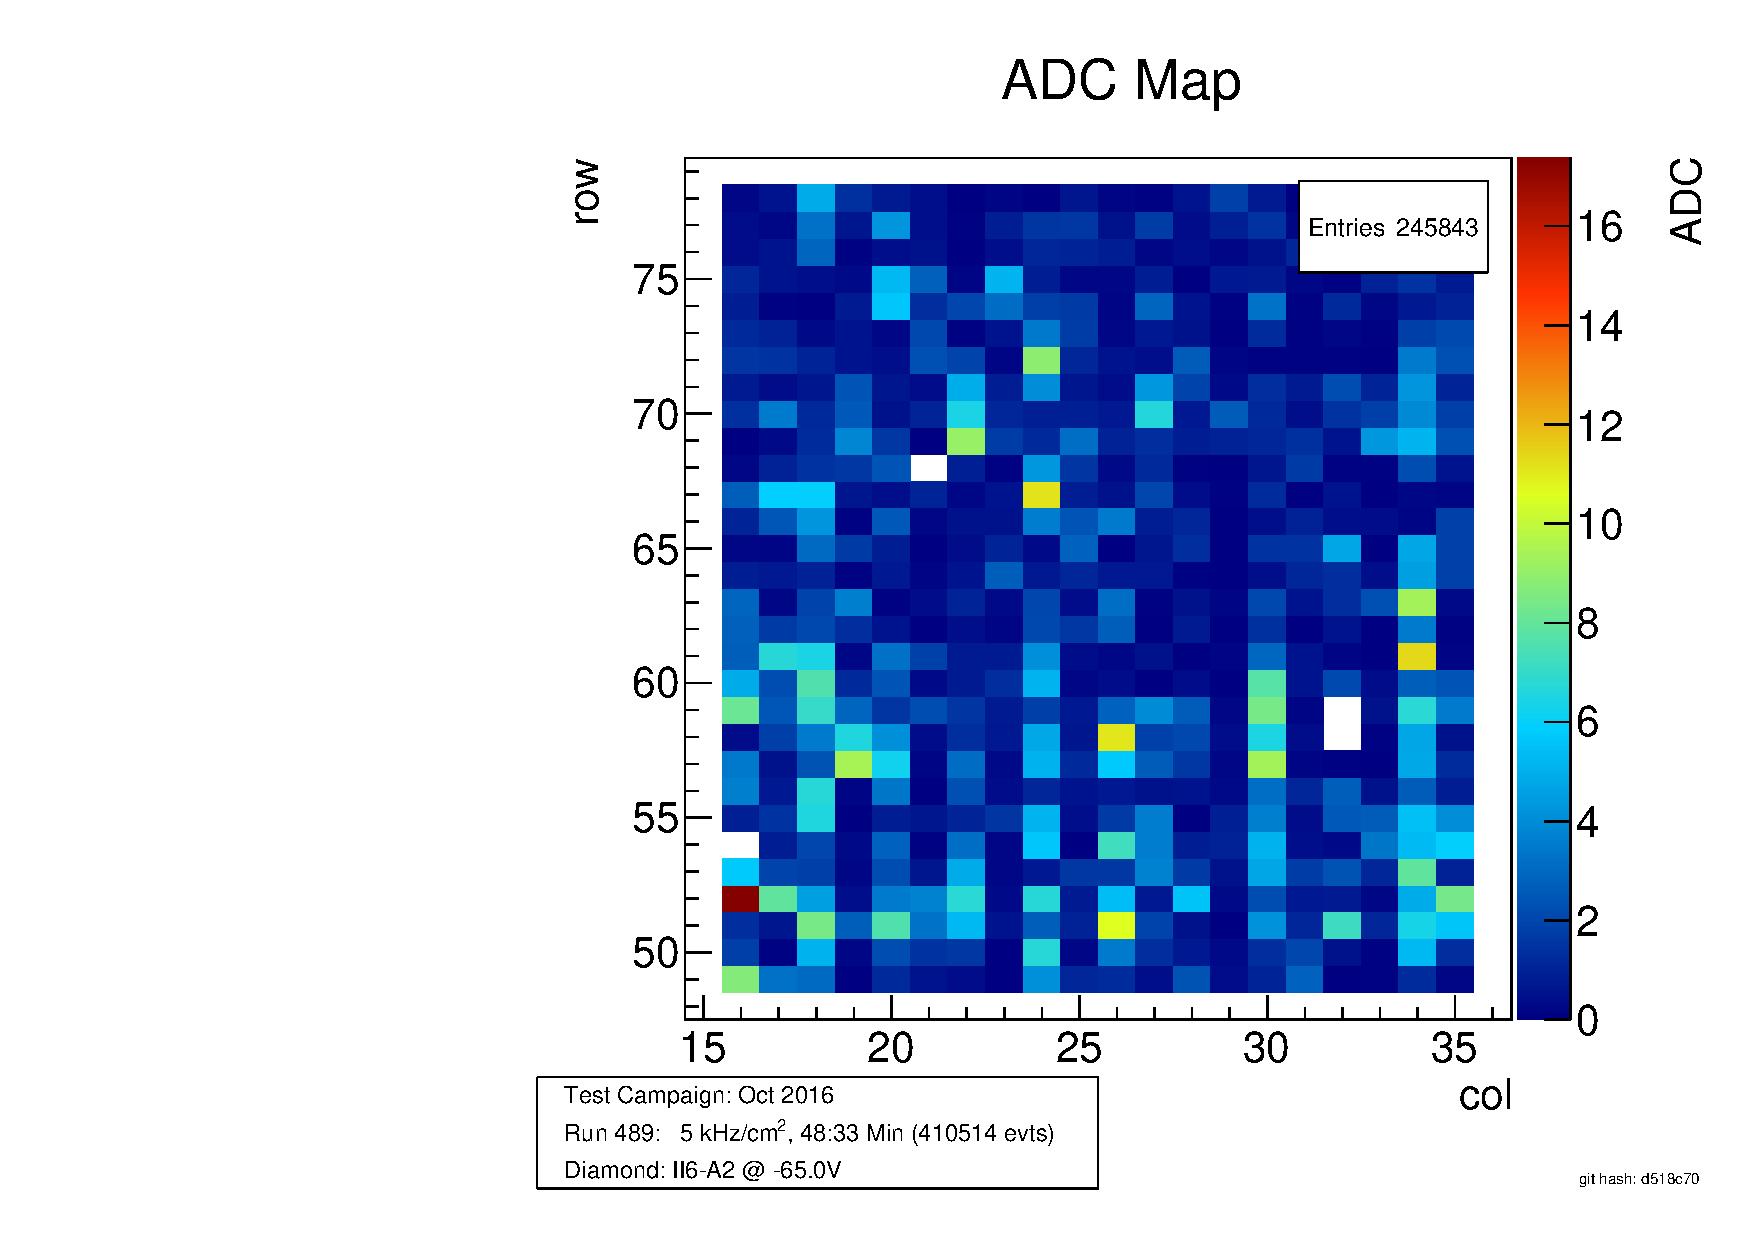
\includegraphics[width=.53\textheight, angle=-90]{AdcMapRaw}
			\caption{raw adc map}
		\end{subfigure}
	\end{figure}\vspace*{-10pt}
	
	\begin{itemize}
		\itemfill
		\item some hot (6) and dead (6) pixels in the detector (total 600 pixels)
		\item very low adc values (\SI{8}{bit} range) \ra most of the values are 0
		\item \textcolor{RedOrange}{\textbf{mistuned chip induced loss of pulse height information}}
	\end{itemize}

\end{frame}
% ================================== 4 ===============================================
\begin{frame}{Pulse Height Distribution}

	\vspace*{-10pt}
	\begin{figure} 
		\begin{center}
			\begin{subfigure}{0.48\textwidth}  
				\centering 
				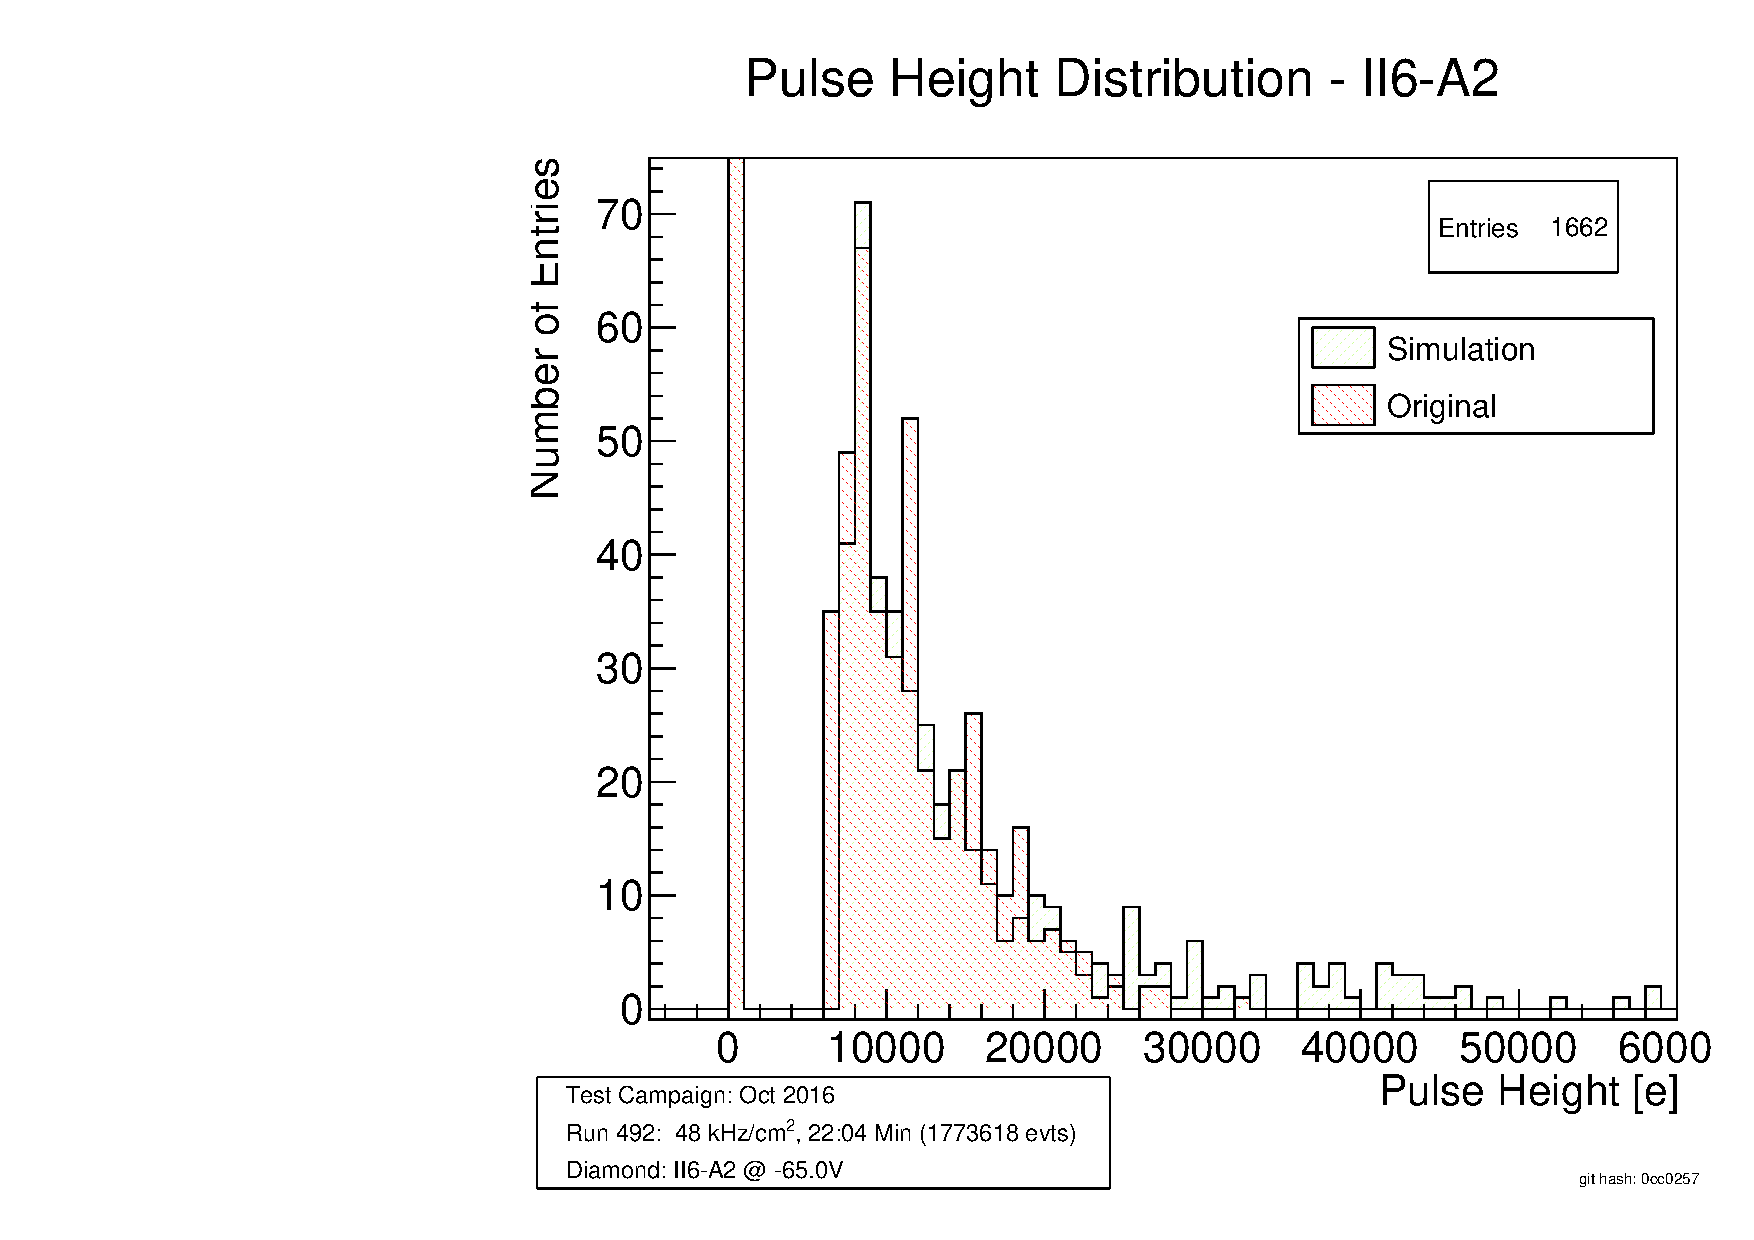
\includegraphics[height=.5\textheight, angle=-90]{Sim2}
				\caption{simulation of Landau with threshold} 	
			\end{subfigure}
			\begin{subfigure}{0.48\textwidth} 
				\centering 
				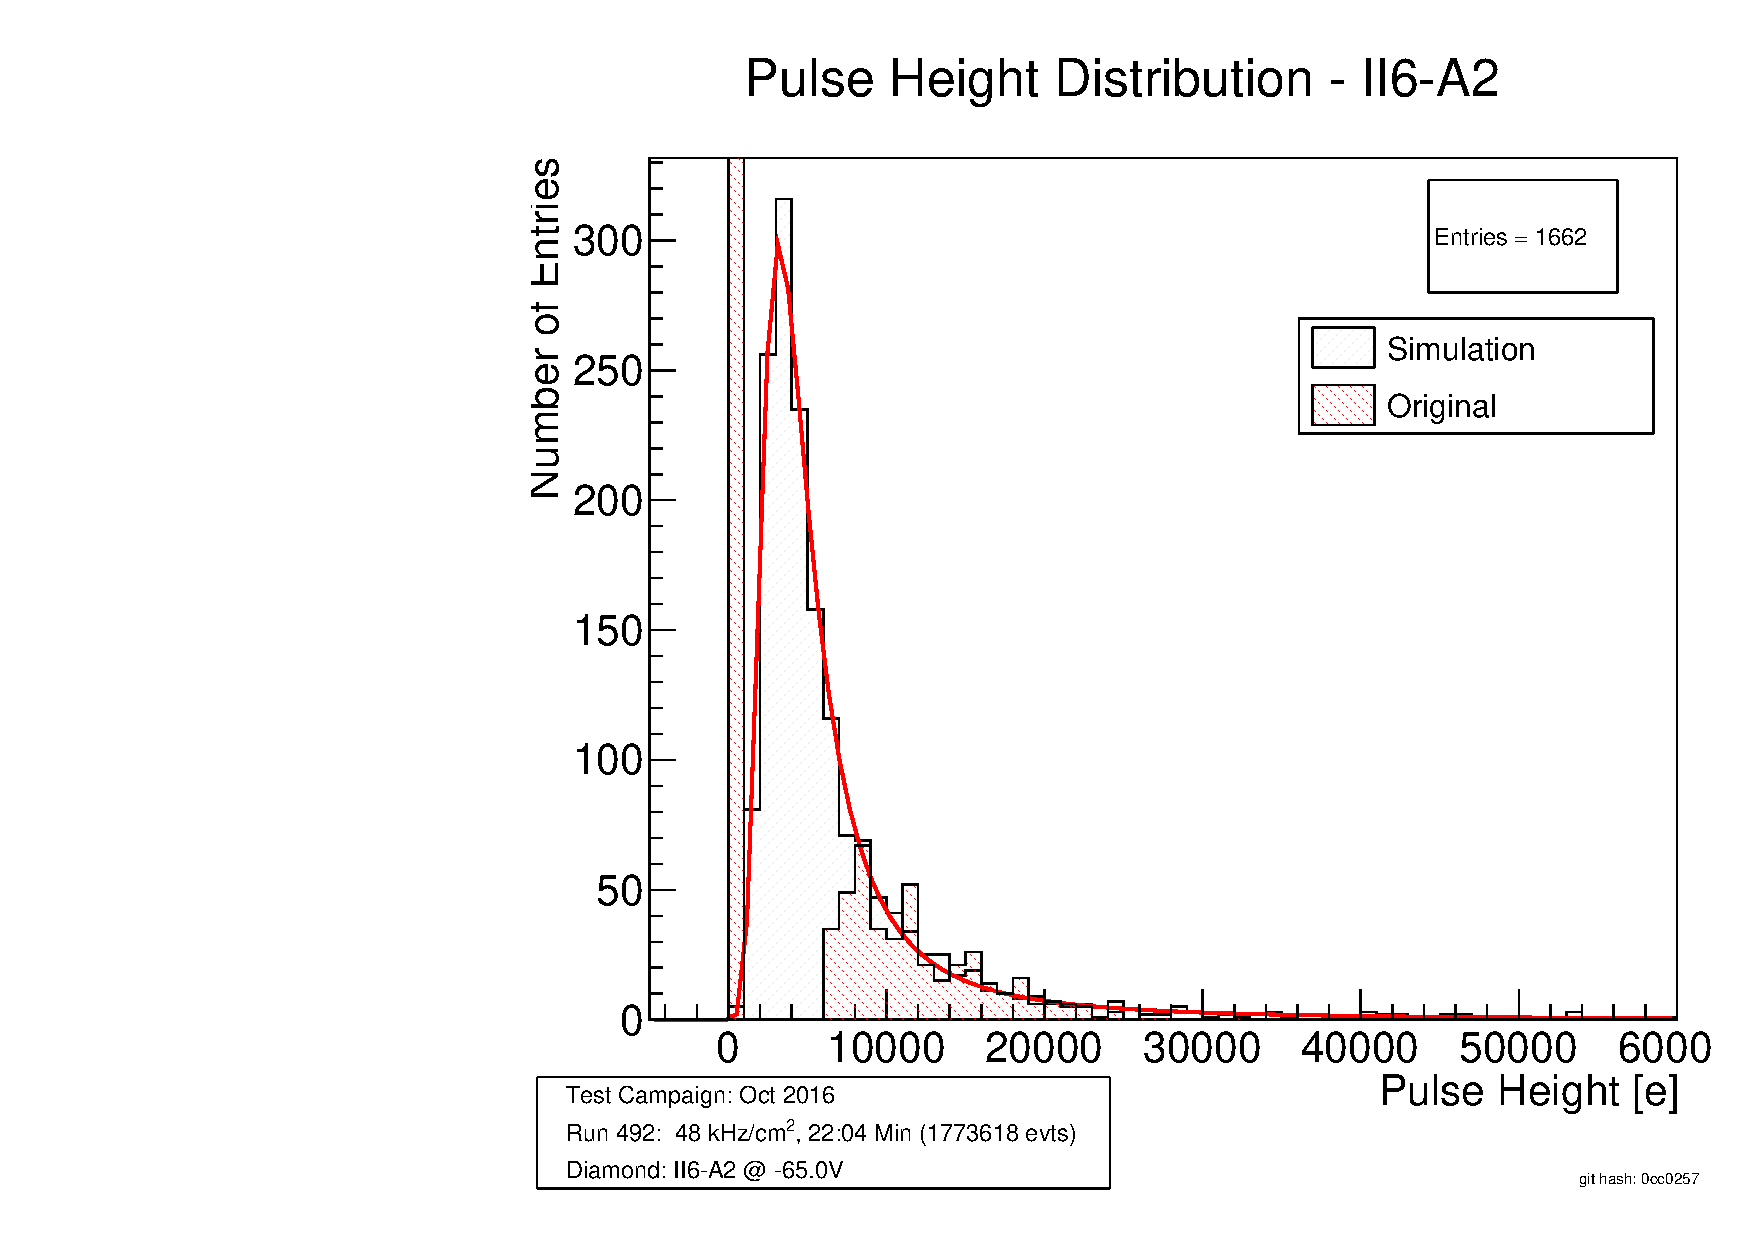
\includegraphics[height=.5\textheight, angle=-90]{Sim3}
				\caption{full distribution with fit} 	
			\end{subfigure} 
		\end{center}
	\end{figure}
	
	\begin{itemize}
		\itemfill
		\item \usebeamercolor[fg]{title} \textbf{mean of the full simulated distribution: \SI{6950}{e}}\usebeamercolor[fg]{normal text}
		\item lower than expected pulse height: \SI{>14000}{e} \ra under investigation
		\item \SI{1.8}{\%} of the events beneath \SI{1500}{e} (pixel threshold)
	\end{itemize}

\end{frame}
% ================================== 5 ===============================================
\begin{frame}{Efficiency Map}

	\vspace*{-10pt}
	\begin{figure} 
		\begin{center}
			\begin{subfigure}{0.48\textwidth}  
				\centering 
				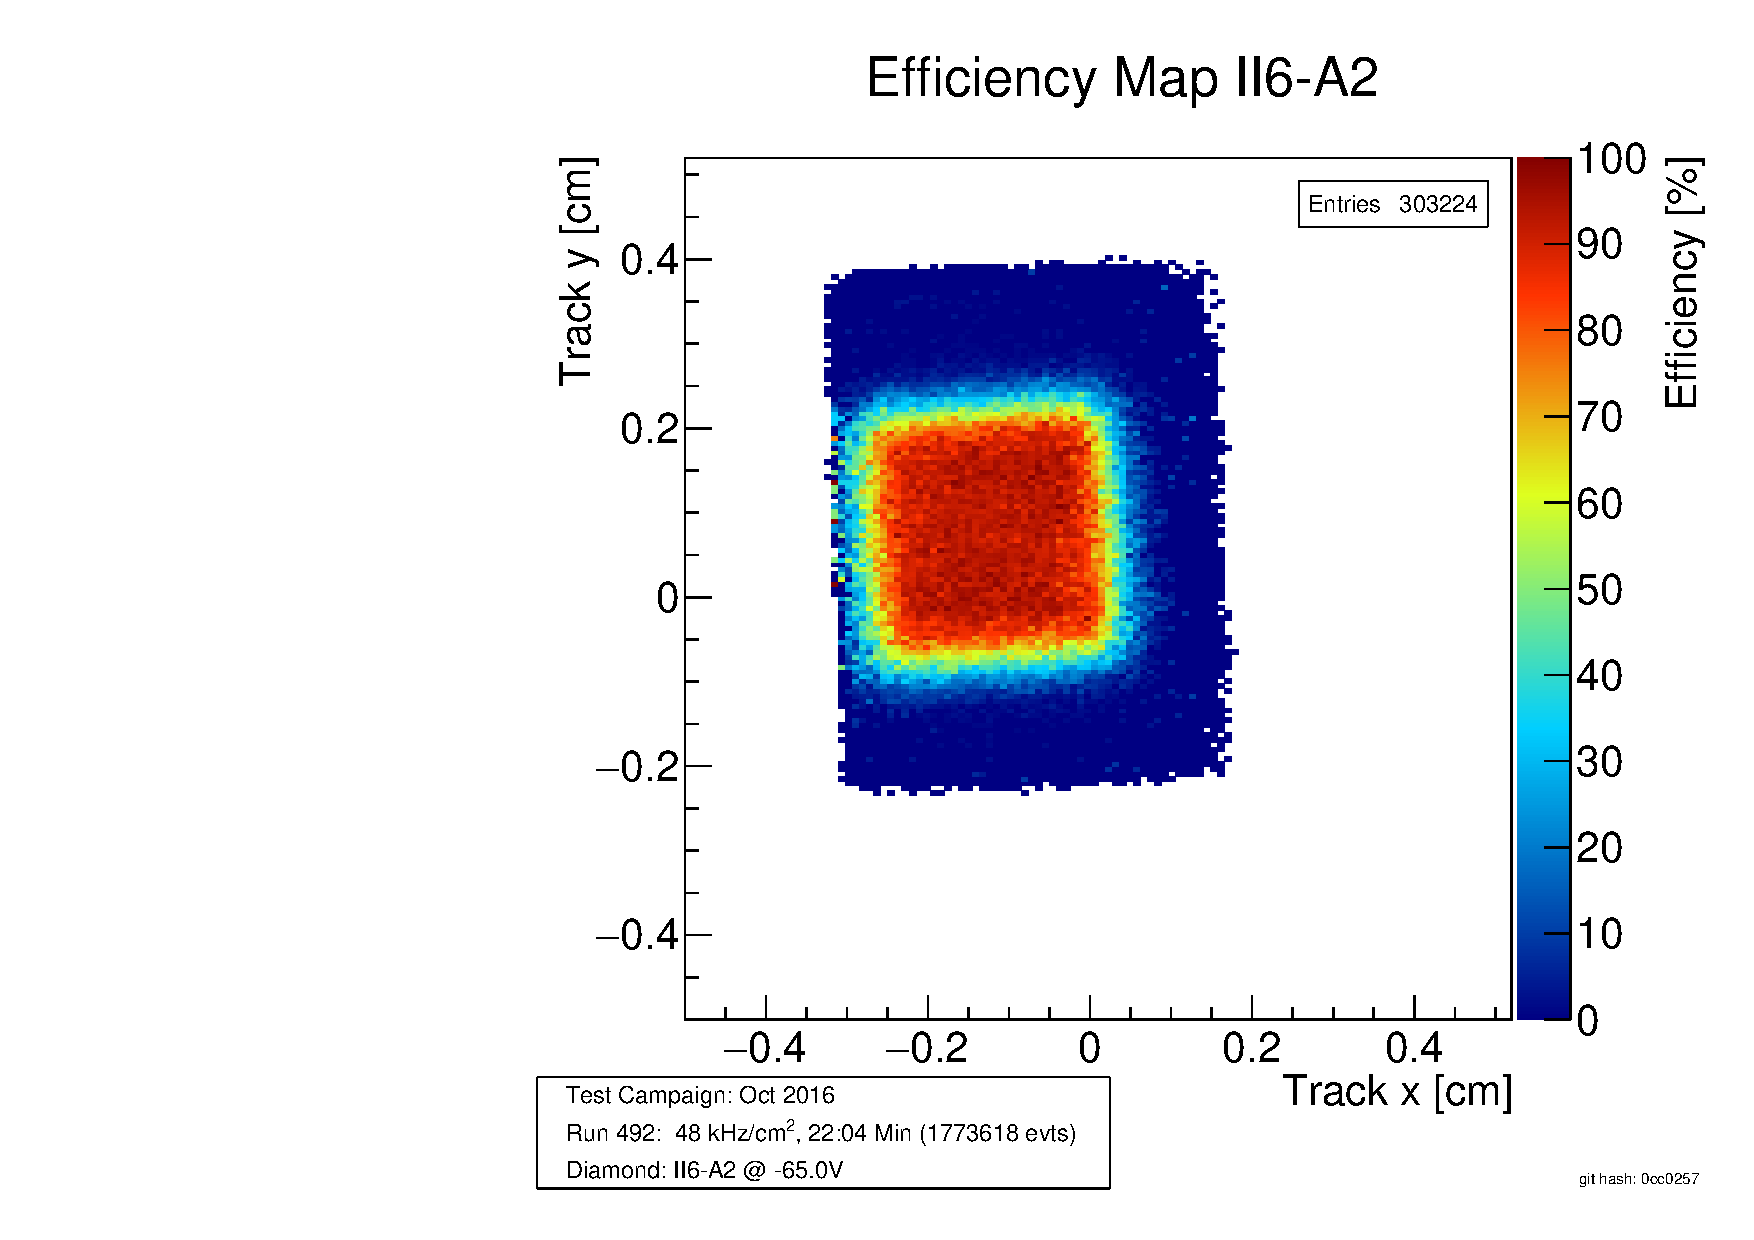
\includegraphics[height=.53\textheight, angle=-90]{EffMap}
				\caption{II6-A2} 	
			\end{subfigure}
			\begin{subfigure}{0.48\textwidth} 
				\centering 
				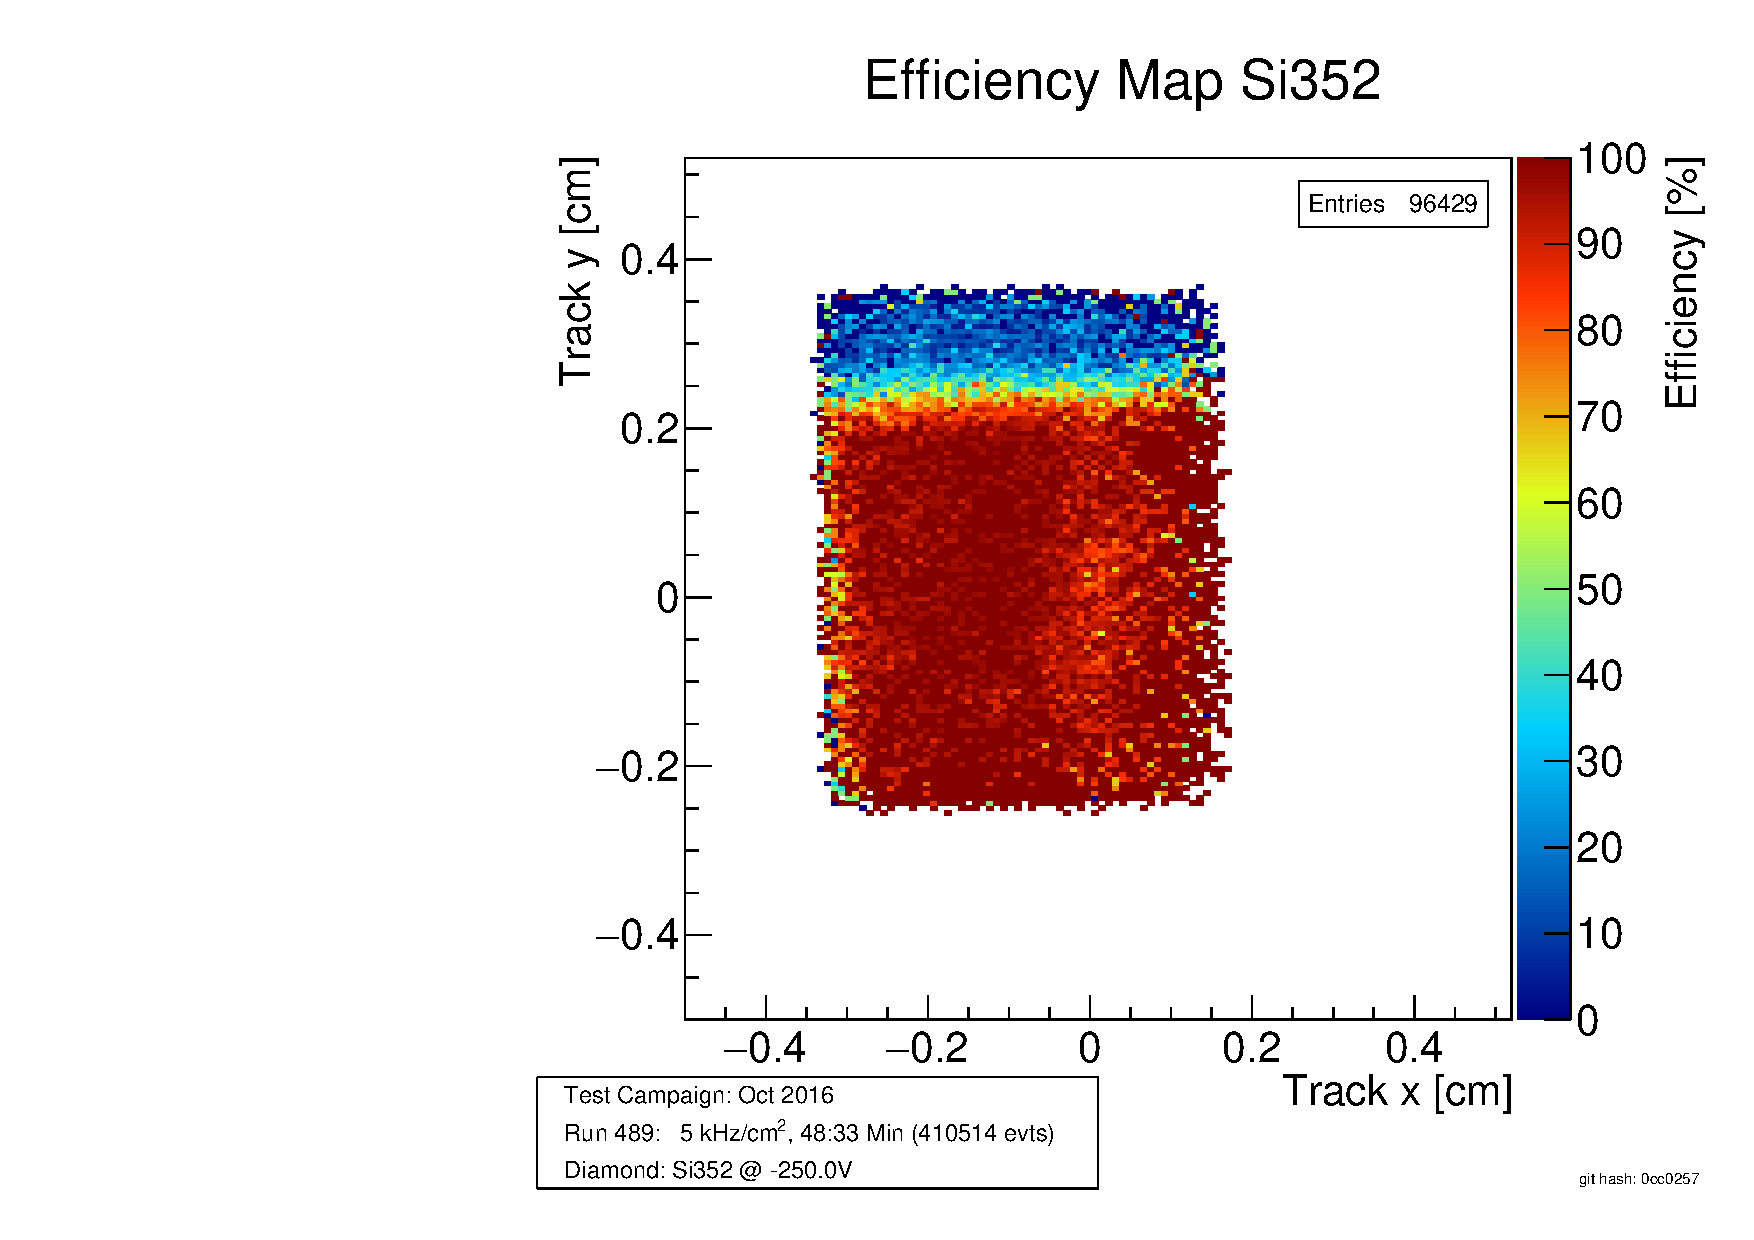
\includegraphics[height=.53\textheight, angle=-90]{EffMapSil}
				\caption{Si352 - reference} 	
			\end{subfigure} 
		\end{center}
	\end{figure}
	
	\begin{itemize}
		\itemfill
		\item percentage of valid hits at estimated hit position by tracking
		\item total area: unmasked area of the trigger planes
		\item central region highly efficient
	\end{itemize}

\end{frame}
% ================================== 6 ===============================================
\begin{frame}{Efficiency vs. Time}

	\vspace*{-10pt}
	\begin{figure} 
		\begin{center}
			\begin{subfigure}{0.48\textwidth}  
				\centering 
				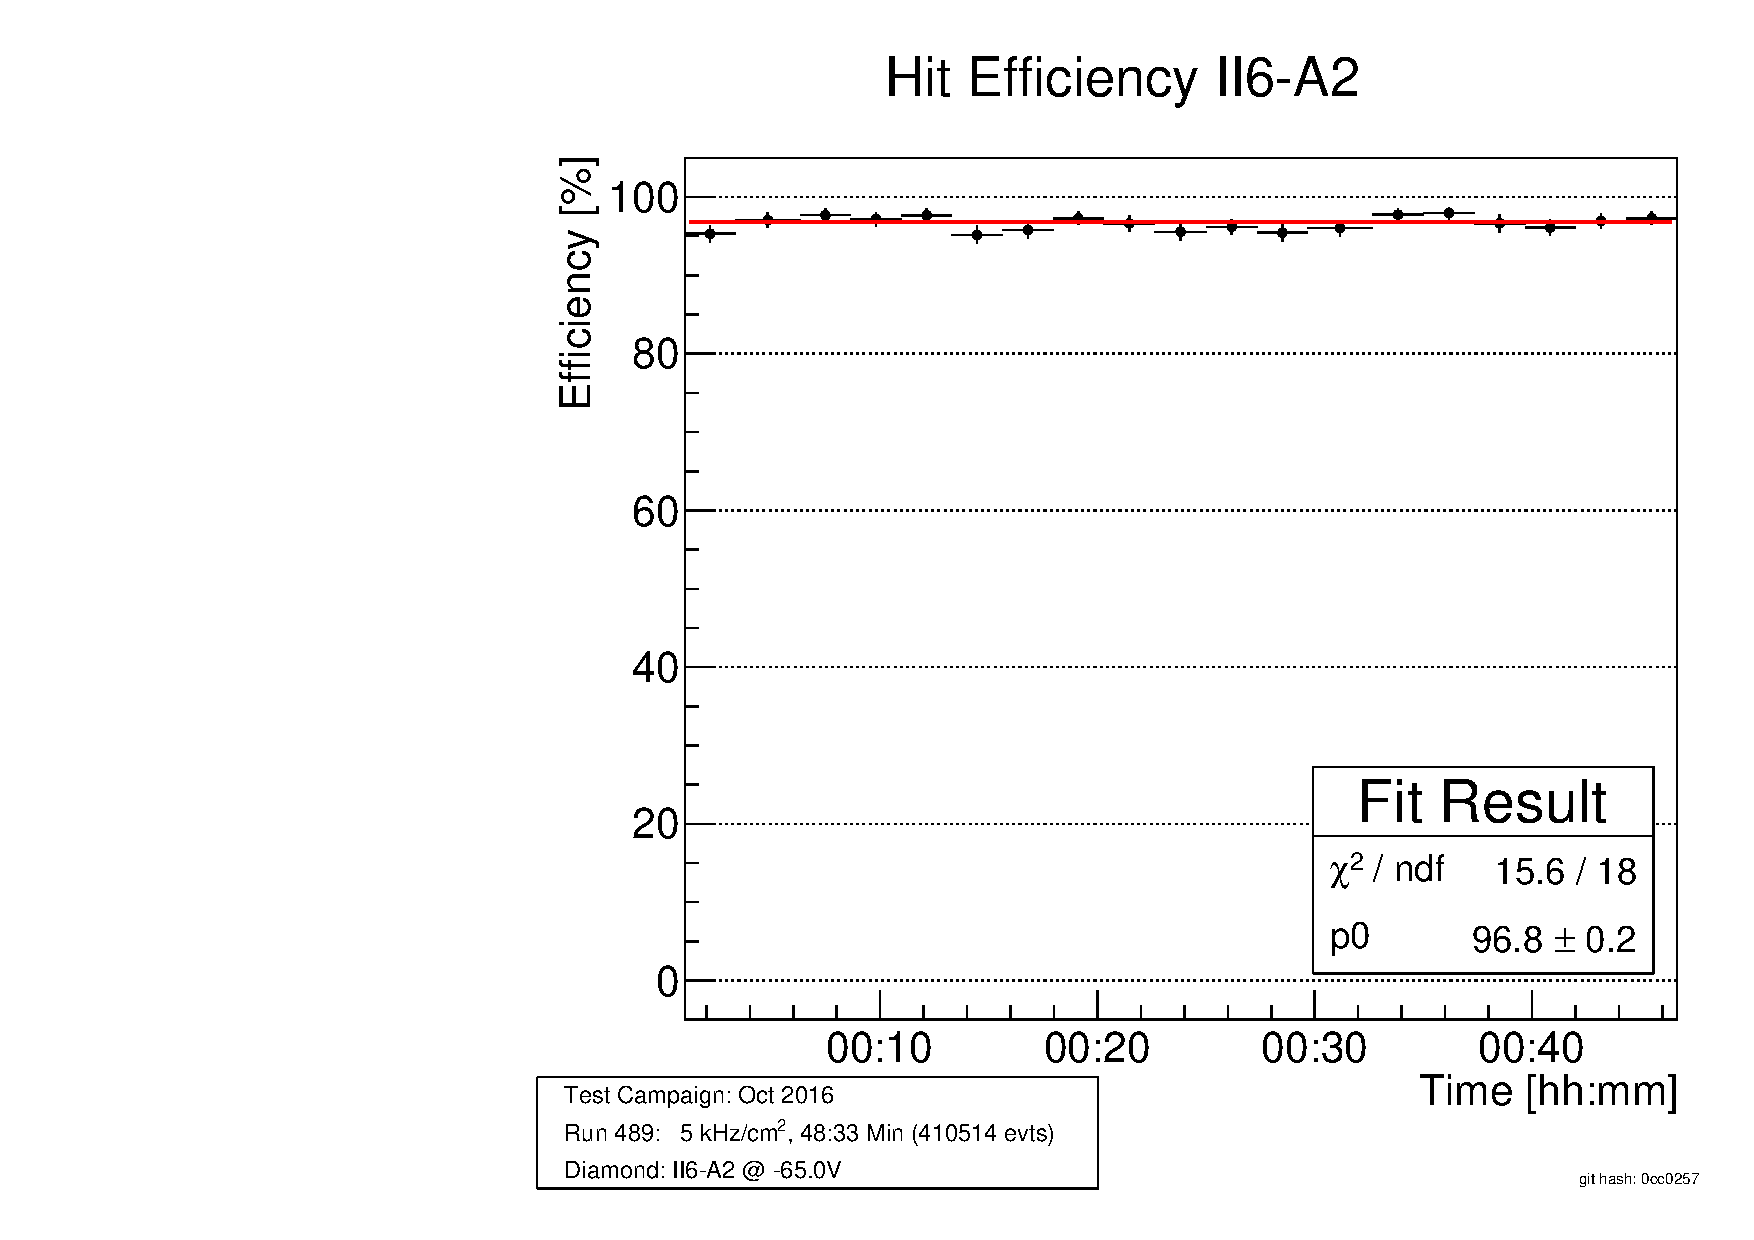
\includegraphics[height=.53\textheight, angle=-90]{EffDiaCut}
				\caption{II6-A2} 	
			\end{subfigure}
			\begin{subfigure}{0.48\textwidth} 
				\centering 
				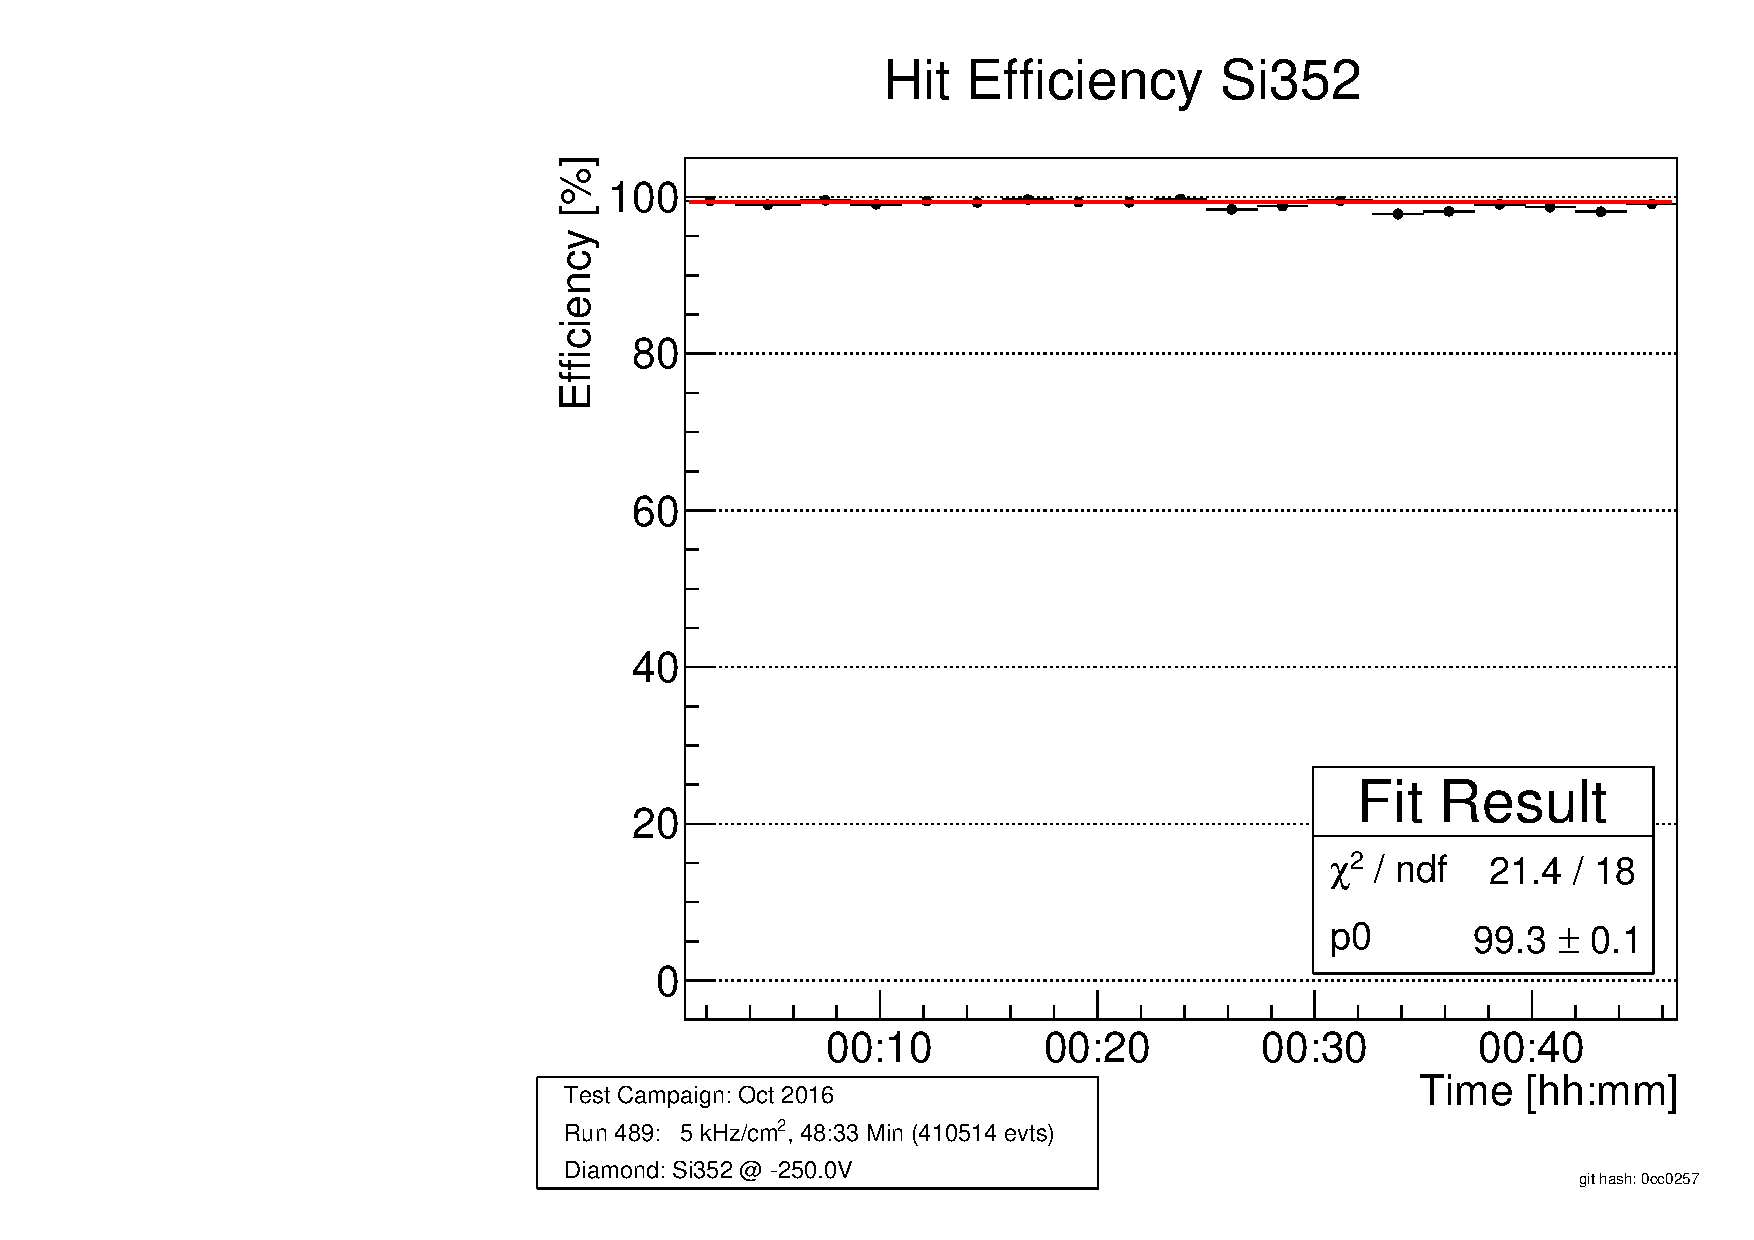
\includegraphics[height=.53\textheight, angle=-90]{EffSilCut}
				\caption{Si352 - reference} 	
			\end{subfigure} 
		\end{center}
	\end{figure}
	
	\begin{itemize}
		\itemfill
		\item \usebeamercolor[fg]{title} \textbf{mean efficiency of the II6-A2: \SI{\sim97}{\%}}\usebeamercolor[fg]{normal text}
		\item mean efficiency of the silicon reference: \SI{\sim99}{\%}
		\item undetected hits likely below pixel threshold \ra agrees well with simulation
	\end{itemize}

\end{frame}
